\subsection*{SARS}
  Since SARS lacks of valid medicines or vaccines, measures to control the 
spread of SARS had to take two major forms: isolation of symptomatic 
individuals and quarantining and close observation of asymptomatic 
individuals \cite{who_sars}. We return to model \eqref{eqn:sars_model} and 
obtain via the forward-backward-sweep method the optimal policies. We use the 
value parameters listed in \Cref{tbl:sars_table}.

  \Cref{fig:figure1sars} displays on the left a likening between the 
controlled total infected population $E + Q + I + J$. Here we contrast the 
resulting dynamics using a constant policy (solid green), 
$\widehat{u}_1 =\num{0.2}$, $\widehat{u}_2 = \num{0.2}$ with the optimal 
quarantine and isolation control (dash orange) policies $u_1$, and $u_2$. At 
left, we see that in order to minimize the total infected individuals, optimal 
control quarantine $u_1$ is at its upper bound during more than \SI{150}{days}, 
then $u_1$ is steadily decreased to the lower bound. Optimal control isolation 
$u_2$ stays at its  upper bound about \SI{70}{days} and then steadily decreases 
to the lower bound over the rest simulated time.

\begin{table}[H]
    \begin{center}
      \begin{tabular}{@{}rlrl@{}}
        \toprule
        \multicolumn{4}{c}{\bf{Parameters values}}
        \\
        \midrule
        $\beta$
          & \num{0.2}
          & $d_1$, $d_2$
          & \num{0.0079}, \num{0.0337}
        \\
        $\varepsilon_E$, 
        $\varepsilon_Q$,
        $\varepsilon_J$
          & \num{0.3}, \num{0.0}, \num{0.1}
          &
          $k_1$, $k_2$ 
          & 
            \num{0.1},
            \num{0.125}
          \\
        $\mu$
          & \num{0.000034}
        \\
        $\Lambda$
          & $\mu N$
        \\
        $p$
          & \num{0.0}
        \\
        $\sigma_1$, $\sigma_2$
          & \num{0.0337}, \num{0.0386}
          && \multicolumn{1}{c}{\bf{Initial conditions}}
        \\
        \cmidrule{4-4}
          &&& $S(0)=\num{12e6}$, $E(0)=1565$,
         \\
        $t_f$
          & $\SI{1.0}{year}$
          && $Q(0)=292$, $I(0)=\num{695}$,
        \\
        Step size
        & $dt=\SI{1.0}{day}$
        && $J(0)=\num{326}$, $R(0)=\num{20}$
        \\
        $u_i$ bounds
          & \num{.05}, \num{0.5}
        \\
        $B_1$, $B_2$, $B_3$, $B_4$
        & \num{1.0}, \num{1.0}, \num{1.0}, \num{1.0}
        \\
        $C_1$, $C_2$
        & \num{300}, \num{600}
        \\
        \bottomrule
      \end{tabular}
     \caption{Parameter description for the SARS model
     \eqref{eqn:sars_model}.}
     \label{tbl:sars_table}
     \end{center}
\end{table}

\begin{figure}[t]
  \centering
  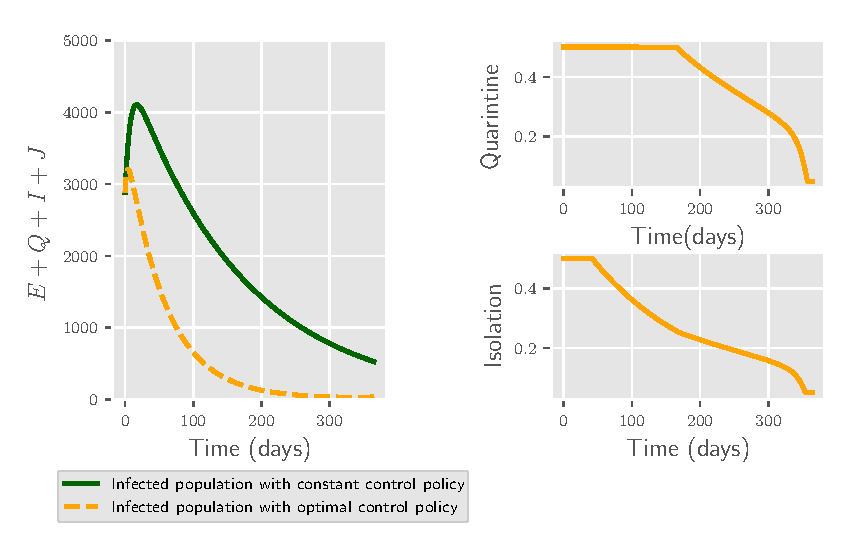
\includegraphics{Figures/figure_1_sars}
  \caption{At left, a likening of the whole infected population
  without constant control and under the optimal policy. }
  \label{fig:figure1sars}
\end{figure}

\begin{figure}[H]
  \centering
  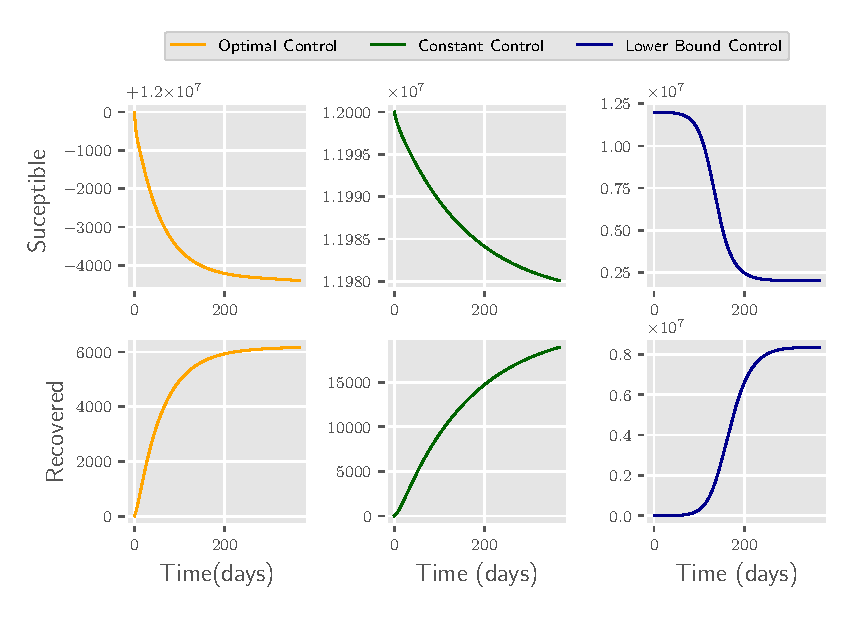
\includegraphics{Figures/figure_2_sars}
  \caption{Susceptible and recover populations under
  optimal, constant and lower bound policies.}
  \label{fig:figure2sars}
\end{figure}

\begin{figure}[H]
  \centering
  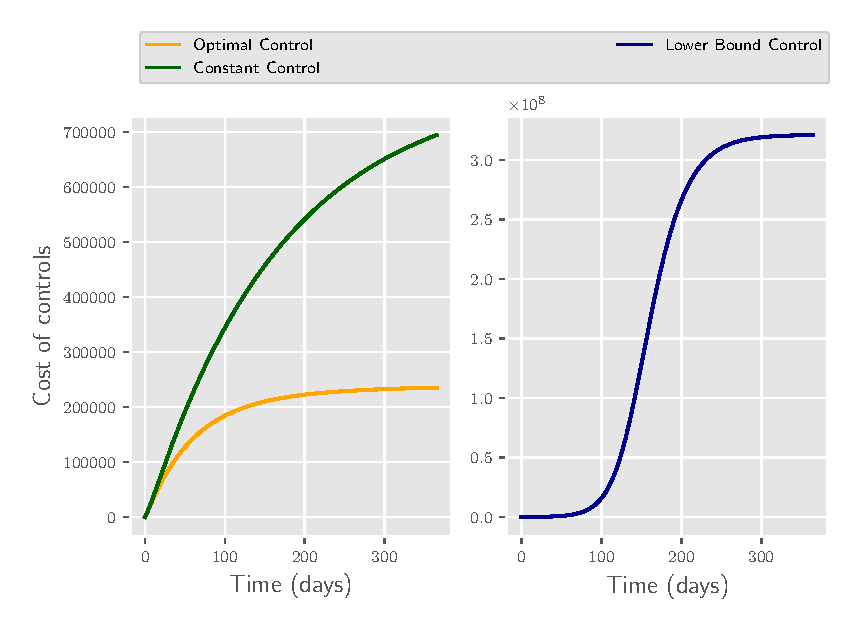
\includegraphics{Figures/figure_3_sars}
  \caption{
    Cost of control-disease for the optimal, constant and lower bound
    policies, see \Cref{eqn:sars_cost}.
  }
  \label{fig:figure3sars}
\end{figure}

\Cref{fig:figure2sars} contrasts the evolution of the dynamics controlled with
the optimal policy, a constant policy 
$\widehat{u}_1 = \widehat{u}_2=\num{0.2}$ and the lower bound policy,
$\bar{u_1} = \bar{u_2} = \num{0.05}$.